%----------------------------------------------------------------
%
%  File    :  vpn_evaluation.tex
%
%  Author  :  Benjamin Wunderling, TU Graz, Austria
% 
%----------------------------------------------------------------

\chapter{Evaluation} \label{chap:Evaluation}

This chapter presents the results of our model learning and model-based fuzzing for \ac{ipsec}-\ac{ike}v1. Model learning results are presented in Section \ref{sec:learnresults}, beginning with the models learned without retransmission-filtering. All model learning and testing took place in a virtual environment using two VirtualBox 6.1 \acp{vm} running standard Ubuntu 22.04 LTS distributions, as described in \ref{chap:Setup}. Next, models of both examined \ac{ipsec} implementations, with retransmission-filtering enabled, are presented and discussed, highlighting differences between the models of the two \ac{ipsec} implementations. The presentation of learned models is followed by a comparison of the two used learning algorithms, $L^*$ and $KV$, as well as the discussion of a library error found during learning. Finally, the fuzzing results for both \ac{ipsec} servers are presented and discussed in Section \ref{sec:fuzzresults}, comparing the various methods of input-sequence generation introduced in Chapter~\ref{chap:Fuzzing}.

\iffalse
\section{Environment Setup} \label{sec:env}
% describe VMs, IPsec server software, configuration etc
All model learning and testing took place in a virtual environment using two VirtualBox 6.1 \acp{vm} running standard Ubuntu 22.04 LTS distributions. Both \acp{vm} were allotted \SI{4}{\giga\byte} of memory and one CPU core. All inter-\ac{vm} communication took place in an isolated virtual network to eliminate possible external influences. During learning and fuzzing, all power saving options and similar potential causes of disruptions were disabled. Additionally, the \ac{ipsec} server was restarted before each learning attempt to ensure identical starting conditions. One \ac{vm} was designated as the initiator and one as the responder to create a typical client-server setup. We chose the open source \ac{ipsec} implementation strongSwan~\cite{software:strongSwan} as our \ac{sul}. The strongSwan server was installed on the responder \ac{vm} and set to listen for incoming connections from the initiator \ac{vm}. We used the strongSwan version US.9.5/K5.15.0-25-generic, installed using the default Ubuntu package manager, apt. The strongSwan server was configured to use \acp{psk} for authentication and default recommended security settings. Additionally, it was configured to allow unencrypted notification messages, which were used to reset the connection during the learning process. Our strongSwan configuration files can be found in Appendix~\ref{app::dot}. The Python library \textsc{AALpy}~\cite{software:aalpy} version 1.2.9 was used in conjunction with the packet manipulation library Scapy\footnote{\url{https://scapy.net/}}, version 2.4.5, in order to learn a model of the \ac{sut}. Significant effort was put into expanding the \ac{isakmp} Scapy module to support all packets required for \ac{ipsec} as the module lacked many features out-of-the-box. The provided Python script, \emph{IPSEC\_IKEv1\_SUL}\footnote{\url{https://github.com/benjowun/VPN-AL}}, demonstrates how \textsc{AALpy} can be used in conjunction with our custom mapper to communicate with and learn the model of an \ac{ipsec} server. Figure~\ref{fig:AALSetup} shows a typical learning attempt using two connected \acp{vm}. The right \ac{vm} shows the output of an underway learning attempt, while the left one shows the corresponding strongSwan server logs.
\fi

\section{Learning Results} \label{sec:learnresults}
% section where we show and analyze reference and no filter models including model and statistics
Over the course of our work, we learned a variety of different models of both \ac{ipsec} servers, due to varying retransmission-handling settings and choices of the input alphabet. As our \ac{sul} had some issues with non-determinism while retransmissions were enabled, one major differentiating factor in our models is whether retransmission-filtering was enabled for the learning process. This had a significant impact on the resulting learned model, with the version without filtering boasting more than twice the number of states than the one with. Additionally, even when using the methods to combat non-determinism described in Section \ref{sec:nondet}, the resulting models still occasionally differed when not filtering out retransmissions. Therefore, the non-filtered models were not used for fuzzing, as a completely deterministic model was desired to serve as our baseline when fuzzing the \ac{sut}.

The following sections first introduce the most relevant metrics used to evaluate the learned models. Next, the two most commonly learned models without retransmission-filtering, both learned from a Linux strongSwan U5.9.5 server, are presented. Finally, models of both servers using the basic and extended input alphabets, with retransmission-filtering enabled, are presented. All models were learned using both the $KV$ and $L^*$ learning algorithms. Error codes have been simplified for better readability and DOT files of all models are provided in Appendix~\ref{app::dot}, as well as in the supplementary material\footnote{\url{https://github.com/benjowun/VPN-AL}}. Note that \textsc{AALpy} refers to output queries as membership queries.

\newpage

\subsection{Learning Metrics} \label{subsec:metrics}
The comparison of learned models and model learning algorithm performance in sections \ref{subsec:models} and \ref{subsec:comp_kv_lstar} is based largely on the following metrics, saved during the model learning process.

\subsubsection*{Steps}
Steps refers to the number of inputs executed on the \ac{sul}. Referred to as steps, input steps or inputs interchangeably.

\subsubsection*{Queries}
Queries refers to the amount of queries sent during state exploration (output queries) or during conformance checking (equivalence queries). \textsc{AALpy} supports speeding up model learning by using caching to reduce the number of required output queries. 

\subsubsection*{Runtime}
Runtime refers to the time it took to learn the model. It is further split into state exploration and conformance checking runtimes. Runtime directly correlates to the number of input steps and queries. When given in seconds, the runtime is rounded to the nearest second.


\subsection{Learned strongSwan Models} \label{subsec:models}
Figures \ref{fig:ret_case1} and \ref{fig:ret_case2} show the two most commonly learned strongSwan models when not filtering retransmissions. Roughly 80\% of all models learned without retransmission-filtering enabled resulted in one of these two models, which we will refer to as the common models. The other 20\% of models were a non-uniform assortment of outliers, an example of which is given in Figure~\ref{fig:ret_out}. Figure \ref{fig:reference} shows the clean base model learned from the strongSwan \ac{sul} with retransmission-filtering enabled. The strongSwan reference model used for fuzzing is shown in Figure \ref{fig:withfilterwitherrors}, also learned with retransmission-filtering enabled, as well as an expanded input alphabet. Figure \ref{fig:learnedmodellibresimple} shows the clean base model learned from the libreswan server. Figure \ref{fig:learnedmodellibrereference} shows the corresponding libreswan fuzzing reference model. 

The strongSwan runtimes of both learning algorithms for all four models are summarized in tables \ref{tab:runtime_summary_kv} and \ref{tab:runtime_summary_lstar}. All values are averages over multiple learning attempts. Note, that while all listed values are averages, the strongSwan clean base model was learned significantly more often than the other models, making the corresponding statistics the most accurate. This is due to the fact, that these models were used as the basis of the comparison between the $KV$ and $L^*$ learning algorithms, presented in Section~\ref{subsec:comp_kv_lstar}. Consequently, as the learning of strongSwan clean base models served a dual purpose, their learning was prioritized. Other models were learned as often as time and resources allowed, usually around ten times per model. The libreswan runtimes were omitted from the statistics, as a workaround had to be used to reset the \ac{ipsec} host \ac{vm} between output queries, potentially skewing the results. Relevant statistics, such as the number of required input steps (i.e. the number of inputs executed on the \ac{sul}) and queries are still presented. The tables use the following abbreviations:

\begin{enumerate}
	\item States: The number of states in the learned model
	\item TT (s): Total time needed to learn the model (in seconds)
	\item TL (s): Time spent on state exploration (in seconds)
	\item TC (s): Time spent on conformance checking (in seconds)
	\item OQ: Number of output queries sent during the model learning
	\item CT: Size of the conformance testing suite, i.e. the number of performed conformance tests
\end{enumerate}
\newpage
 

\subsubsection*{First Common Model}

The first common model, learned from the strongSwan server, is presented in Figure \ref{fig:ret_case1} and took approximately 52 minutes (3092 seconds) to learn with the $KV$ algorithm, spread over seven learning rounds. The model consists of ten states. Of the 52 minutes total, roughly half were used for state exploration/output queries and the other half for conformance checking, with conformance checking taking slightly longer (1501 vs 1591 seconds). 171 output queries were performed by the learning algorithm in 2047 steps, whereas 100 conformance tests were performed for equivalence checking in 1826 steps.

In contrast, when learned with the $L^*$ algorithm, model learning took almost 85 minutes (5094 seconds) over five learning rounds. Here, the split between state exploration and conformance checking was more distinct, with state exploration taking up approximately 68\% of the total runtime and conformance checking only requiring the remaining 32\% (3489 vs 1605 seconds). 462 output queries (2922 steps) were required compared to the 171 queries of the $KV$ algorithm. Notably, the time needed for conformance checking remained largely the same between the two algorithms, however the difference in state exploration/output queries is quite large. However, conformance checking required only 1379 inputs steps than with the $KV$ algorithm. This behavior is discussed in more detail in Section \ref{subsec:comp_kv_lstar}, which includes a statistical comparison of the two algorithms.

Moving on to an examination of the first common model itself, we can clearly see a separation between the two phases. Phase one completes in state \emph{s3}, and phase two begins right thereafter with the transition from state \emph{s3} to \emph{s4}. While phase one looks very clean and is in fact identical to the model learned with retransmission-filtering enabled, phase two has many unexpected transitions caused by retransmissions. For example, all three transitions from state \emph{s5} to \emph{s7} via \emph{authenticate}, \emph{sa\_main} and \emph{key\_ex\_main}, highlighted in yellow, return a valid \emph{IPSEC SA} response. This should be impossible, as phase one messages are to be ignored while in phase two. However, due to specific timings of retransmissions, our communication interface can occasionally happen to be listening for a server response of a regular phase two communication, when the \ac{sul} sends a retransmission for previous \emph{sa\_quick} message. This causes our framework to treat the received retransmission as the response for the phase two message, when in fact, it is not. We can see multiple incoming and outgoing transitions of state \emph{s4}, highlighted in red, that further exhibit this behavior.
Another noticeable property of the learned automata, is that past state \emph{s2}, no paths lead back to the initial state. This is due to the fact that our input alphabet for this learned model does not include the delete command. Adding \ac{isakmp} delete to the input alphabet creates transitions from every state back to the initial one, but also dramatically increases the runtime and non-deterministic behavior of the \ac{sul}, as even more retransmissions are triggered. While not part of our input alphabet, it could be included in future work.

\subsubsection*{Second Common Model}

The second common model of the strongSwan server, seen in Figure \ref{fig:ret_case2}, took approximately 75 minutes (4507 seconds) to learn using the $KV$ algorithm. The model took nine rounds to learn, and consists of twelve states. Of those 75 minutes, roughly 53\% were used for state exploration/output queries and the other 47\% (2382 vs 2126 seconds). 215 output queries were performed by the learning algorithm, requiring 2219 steps, whereas 120 conformance tests were performed, requiring 1964 steps. 

In contrast, when learned with the $L^*$ algorithm, model learning took significantly longer, running for 125 minutes (7520 seconds) over five learning rounds. Here, the split between state exploration and conformance checking was again very distinct, with state exploration taking up approximately 71\% of the total runtime and conformance checking only requiring the remaining 29\% (5393 vs 2126 seconds). Again, the time needed for conformance checking remained largely the same between the two algorithms, however the difference in state exploration/output queries is even larger, with $L^*$ taking 522 output queries. State exploration required 4225 inputs to complete, whereas conformance checking required 1745.

\begin{figure}[H]
	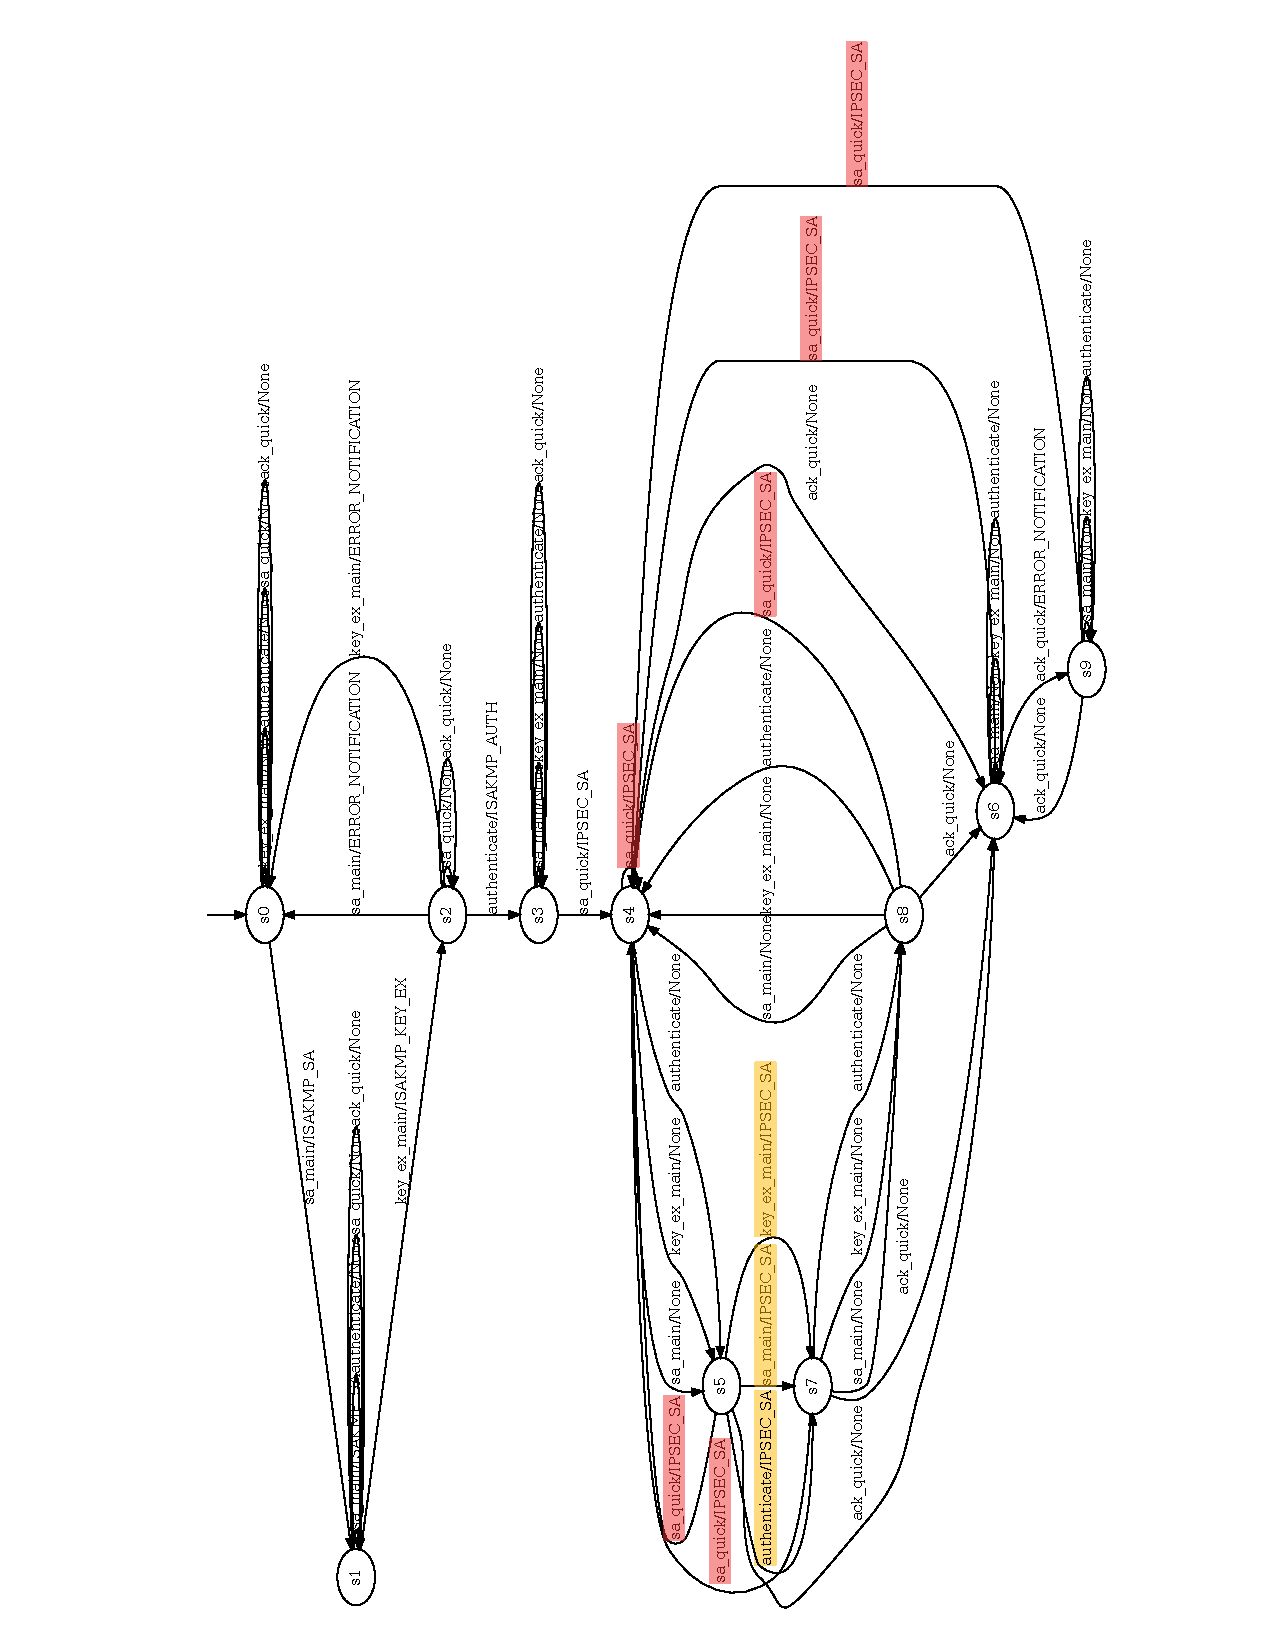
\includegraphics[width=1.1\linewidth]{images/models/retransmissions/retrans_case1_lstar}
	\caption{First commonly learned model of strongSwan server with retransmissions enabled.}
	\label{fig:ret_case1}
\end{figure}

\begin{figure}[H]
	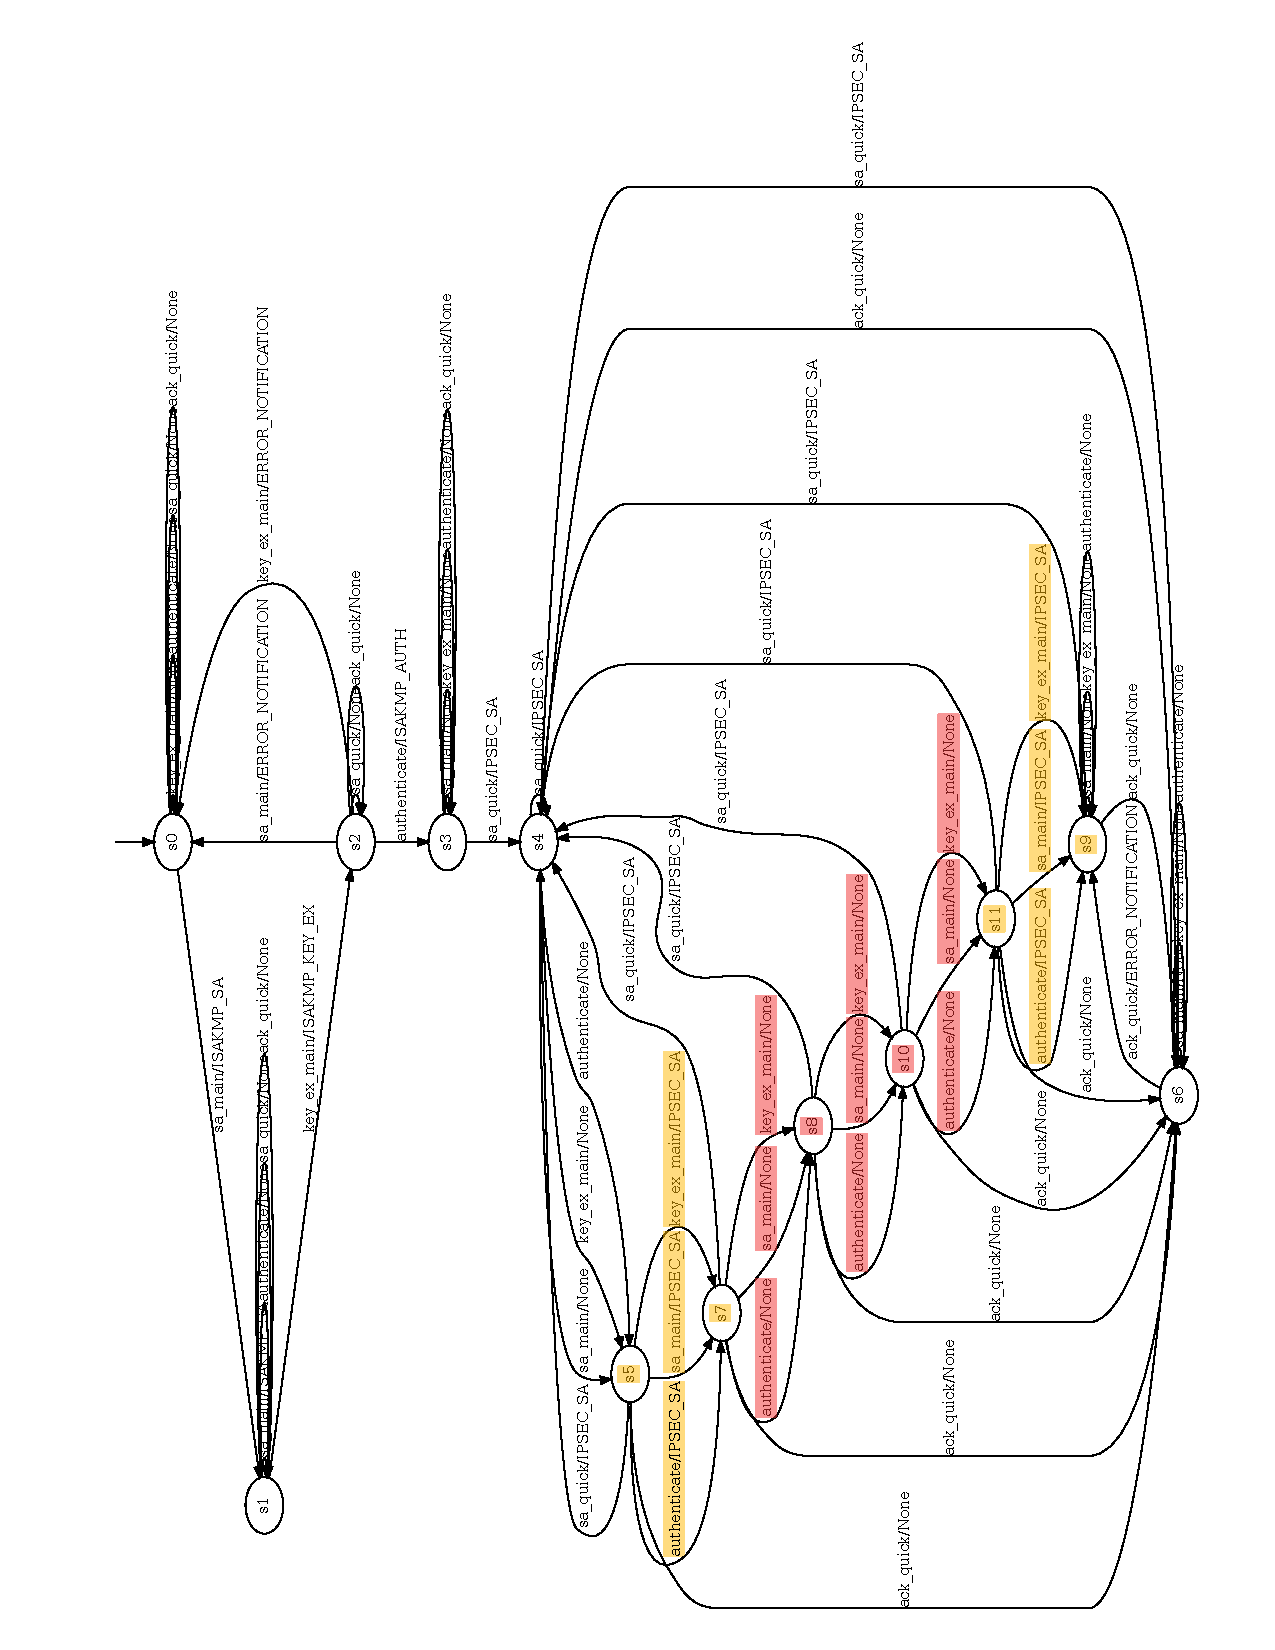
\includegraphics[width=1.1\linewidth]{images/models/retransmissions/retrans_case2_lstar}
	\caption{Second commonly learned strongSwan server model with retransmissions enabled.}
	\label{fig:ret_case2}
\end{figure}

\newpage

Examining the model, we can again see a clear separation between the two phases. Phase one for this model is identical to the previous one, as no retransmission occur there. Same as in Figure \ref{fig:ret_case1}, no paths past state \emph{s2} lead back to the initial state. Phase two shows retransmission-induced strange behavior in the transitions \emph{s5} to \emph{s7}, as well as \emph{s11} to \emph{s9}. The strange behavior is again linked to retransmissions, causing phase one inputs, such as \emph{sa\_main}, to result in the valid phase two outputs, such as \emph{IPSEC SA}. The states \emph{s7} and \emph{s11} are separated by two states that do not exhibit any strange behavior, apart from having identical inputs and outputs. The main difference to the first common model is, that strange behavior occurs in two pairs of states, highlighted in yellow, and that these pairs are separated by two states that do not appear to receive any retransmissions, highlighted in red. This is likely caused by the \ac{sut} sending repeated retransmissions, in the same frequency, allowing for two states in between. 


\subsubsection*{Other outliers}
Figure~\ref{fig:ret_out} shows a sample outlier model of the strongSwan \ac{ipsec} server, learned using the $L^*$ algorithm in approximately 200 minutes (12187 seconds). It consists of 13 states, which were learned over five learning rounds. The runtime was shared between state exploration and conformance checking in a 60/40 split. State exploration took 5188 input steps to complete, whereas conformance checking only took 1847 steps. Unfortunately, due to the random nature of the outliers, this exact model could not be learned using the $KV$ algorithm within the allotted time frame. When model learning the \ac{ipsec} server without enabling retransmission-filtering, roughly 20\% of the learned models differed from the two already presented common models. Figure~\ref{fig:ret_out} shows one such model. They all showcased slight deviations, such as additional states and/or transitions cause by server retransmissions. 

The presented outlier model showcases characteristics of both common models, with states \emph{s5} and \emph{s7} (highlighted in yellow) resembling states \emph{s6} and \emph{s9} of the first common model. Additionally, the central states of the outlier model (highlighted in red) resemble those of the second common model in that it features a long chain of retransmissions allowing otherwise invalid phase one messages in phase two.



\begin{figure}[H]
	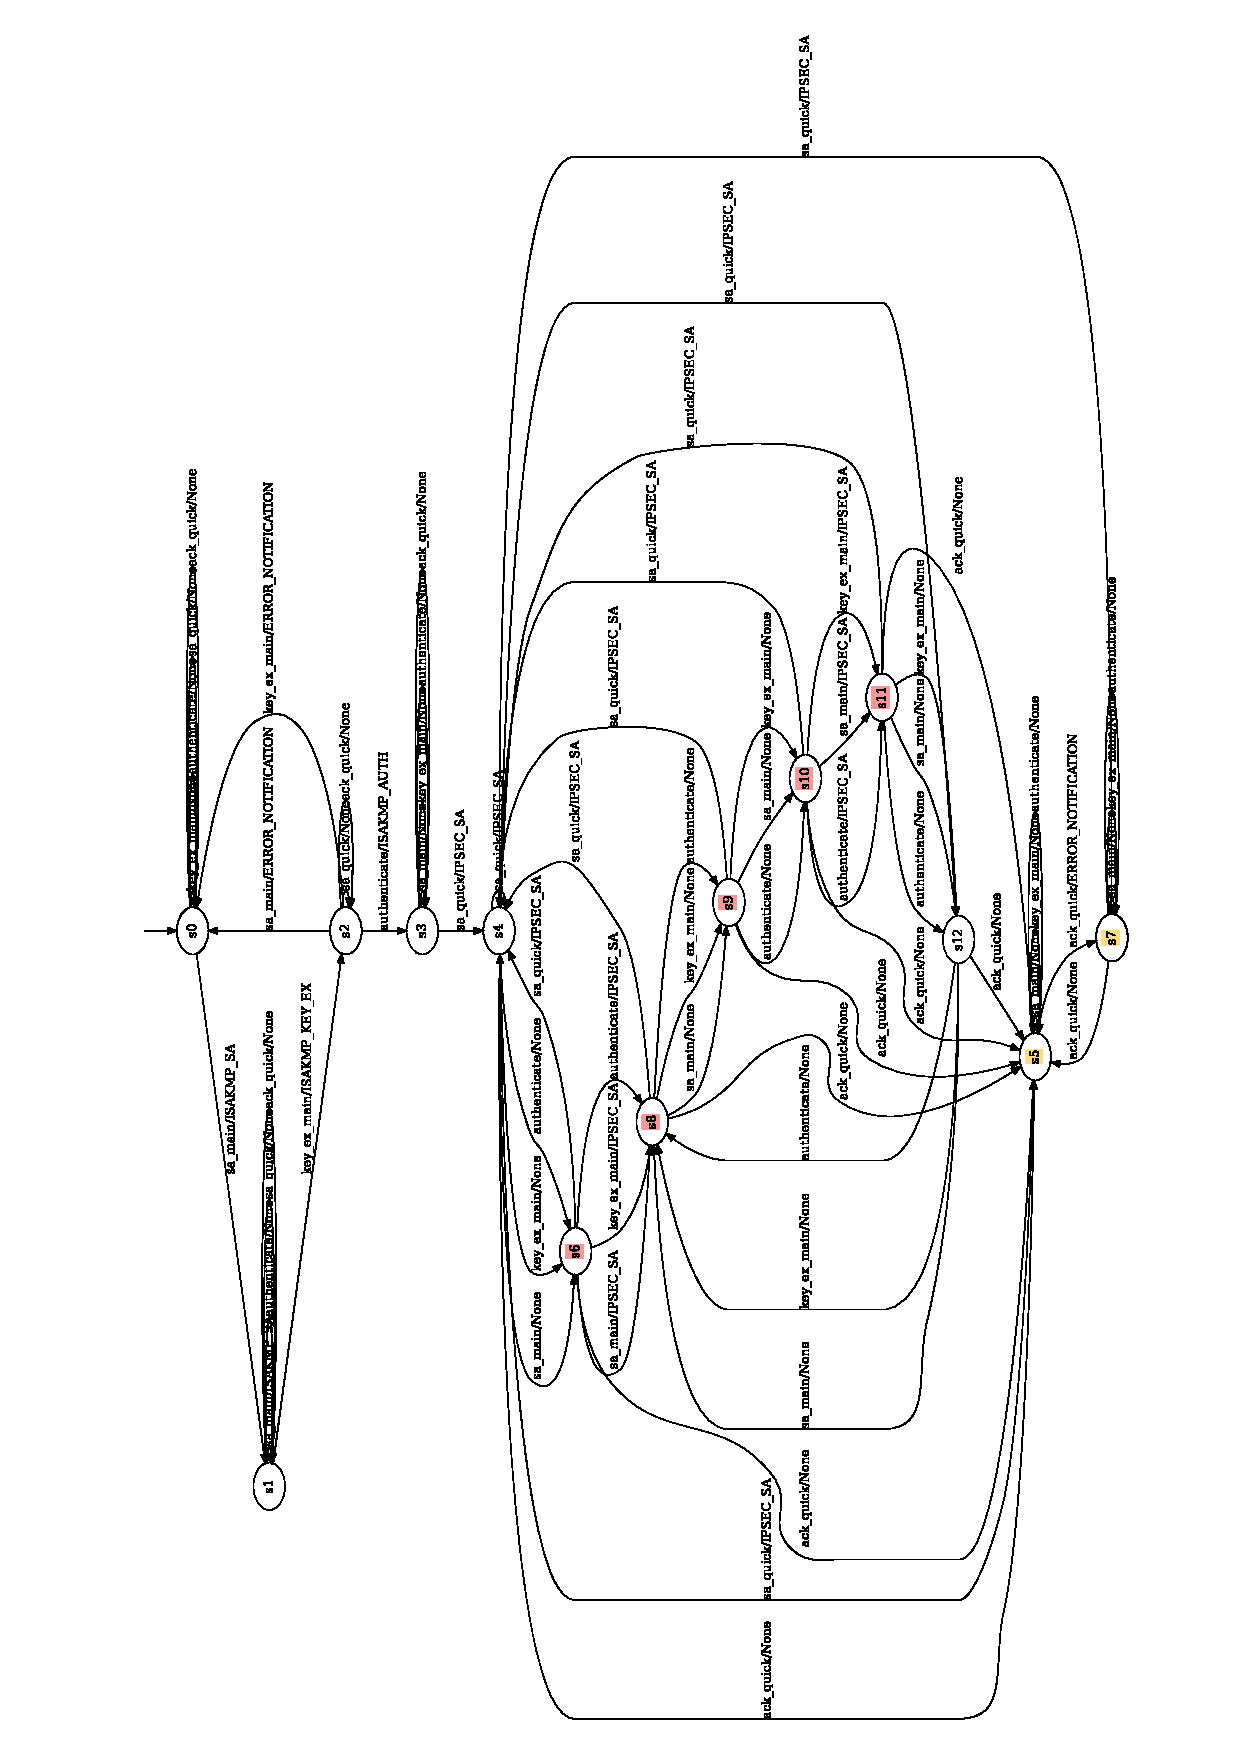
\includegraphics[width=\linewidth]{images/models/retransmissions/outlier_rotated}
	\caption{A rare outlier model, learned with retransmissions enabled.}
	\label{fig:ret_out}
\end{figure}


\subsubsection*{Clean Base Models}

In comparison, when learning the same server implementation with retransmission-filtering enabled, all non-deterministic behavior vanishes and we get the model shown in Figure~\ref{fig:reference} for every learning attempt. The model has only six states and therefore was learned much more quickly than the previous ones, with learning requiring only approximately 21 minutes (1266 seconds) using the $KV$ algorithm. Learning happened over four rounds, taking 676 input steps, where the time was distributed between state exploration and conformance checking in a 40/60 split (519 vs 747 seconds). Conformance checking took an average of 934 input steps to complete. This was the only configuration where the conformance checking took longer than state exploration, as highlighted in Table \ref{tab:runtime_summary_kv}. It does however still have the lowest altogether runtime. In comparison, when learned with the $L^*$ algorithm, learning took roughly 36 minutes (2157 seconds), spread over two learning rounds. Of that time, state exploration required roughly 55\% compared to the 45\% needed for conformance checking (1188 vs 969 seconds), with state exploration requiring 856 and conformance checking requiring only 747 input steps. Compared to $KV$, state exploration/output queries took more than twice the amount of time to complete.\\

\begin{table}[H]
	\centering
	\begin{tabular}{|l|l|l|l|l|l|l|}
		\hline
		\rowcolor[HTML]{C0C0C0} 
		Model     		& States & TT (s)  & TL (s)  & TC (s)  & OQ  & CT  \\ \hline
		First Common 	& 10     & 3092 & 1501 & 1591 & 171 & 100 \\ \hline
		Second Common  	& 12     & 4507 & 2382 & 2126 & 215 & 120 \\ \hline
		Base      		& 6      & 1214 & 480  & 734  & 78  & 60  \\ \hline
		Reference 		& 6      & 1447 & 879  & 568  & 174 & 60  \\ \hline
	\end{tabular}
	\caption{KV Runtimes of all the learned strongSwan models.}
	\label{tab:runtime_summary_kv}
\end{table}

Looking at the resulting model more closely, the first four states are again identical to the previous model. This is due to the fact that the retransmissions are only triggered for phase two messages and since they are our only source of non-determinism, there are no differences here. However, the phase two states look wildly different, showing a streamlined behavior that fits our reference \ac{ike} exchange (see Figure \ref{fig:IKEv1}) almost perfectly. The only small difference lies in the additional state \emph{s5} which loops back to state \emph{s4} with an \emph{IPSEC SA} or \emph{ACK} message. This behavior shows how multiple \ac{ipsec} \acp{sa}, each created from a single IKE SA channel, can be used interchangeably for different traffic flows but not simultaneously. As soon as a new \ac{ipsec} \ac{sa} has been established, another \emph{ACK} message can be sent, to finalize the creation of the new \ac{ipsec} \ac{sa}. In other words, the extra state is there to show that a single \ac{ipsec} \ac{sa} cannot be acknowledged twice, and instead a new \ac{sa} must be created first. 

\begin{figure}[H]
	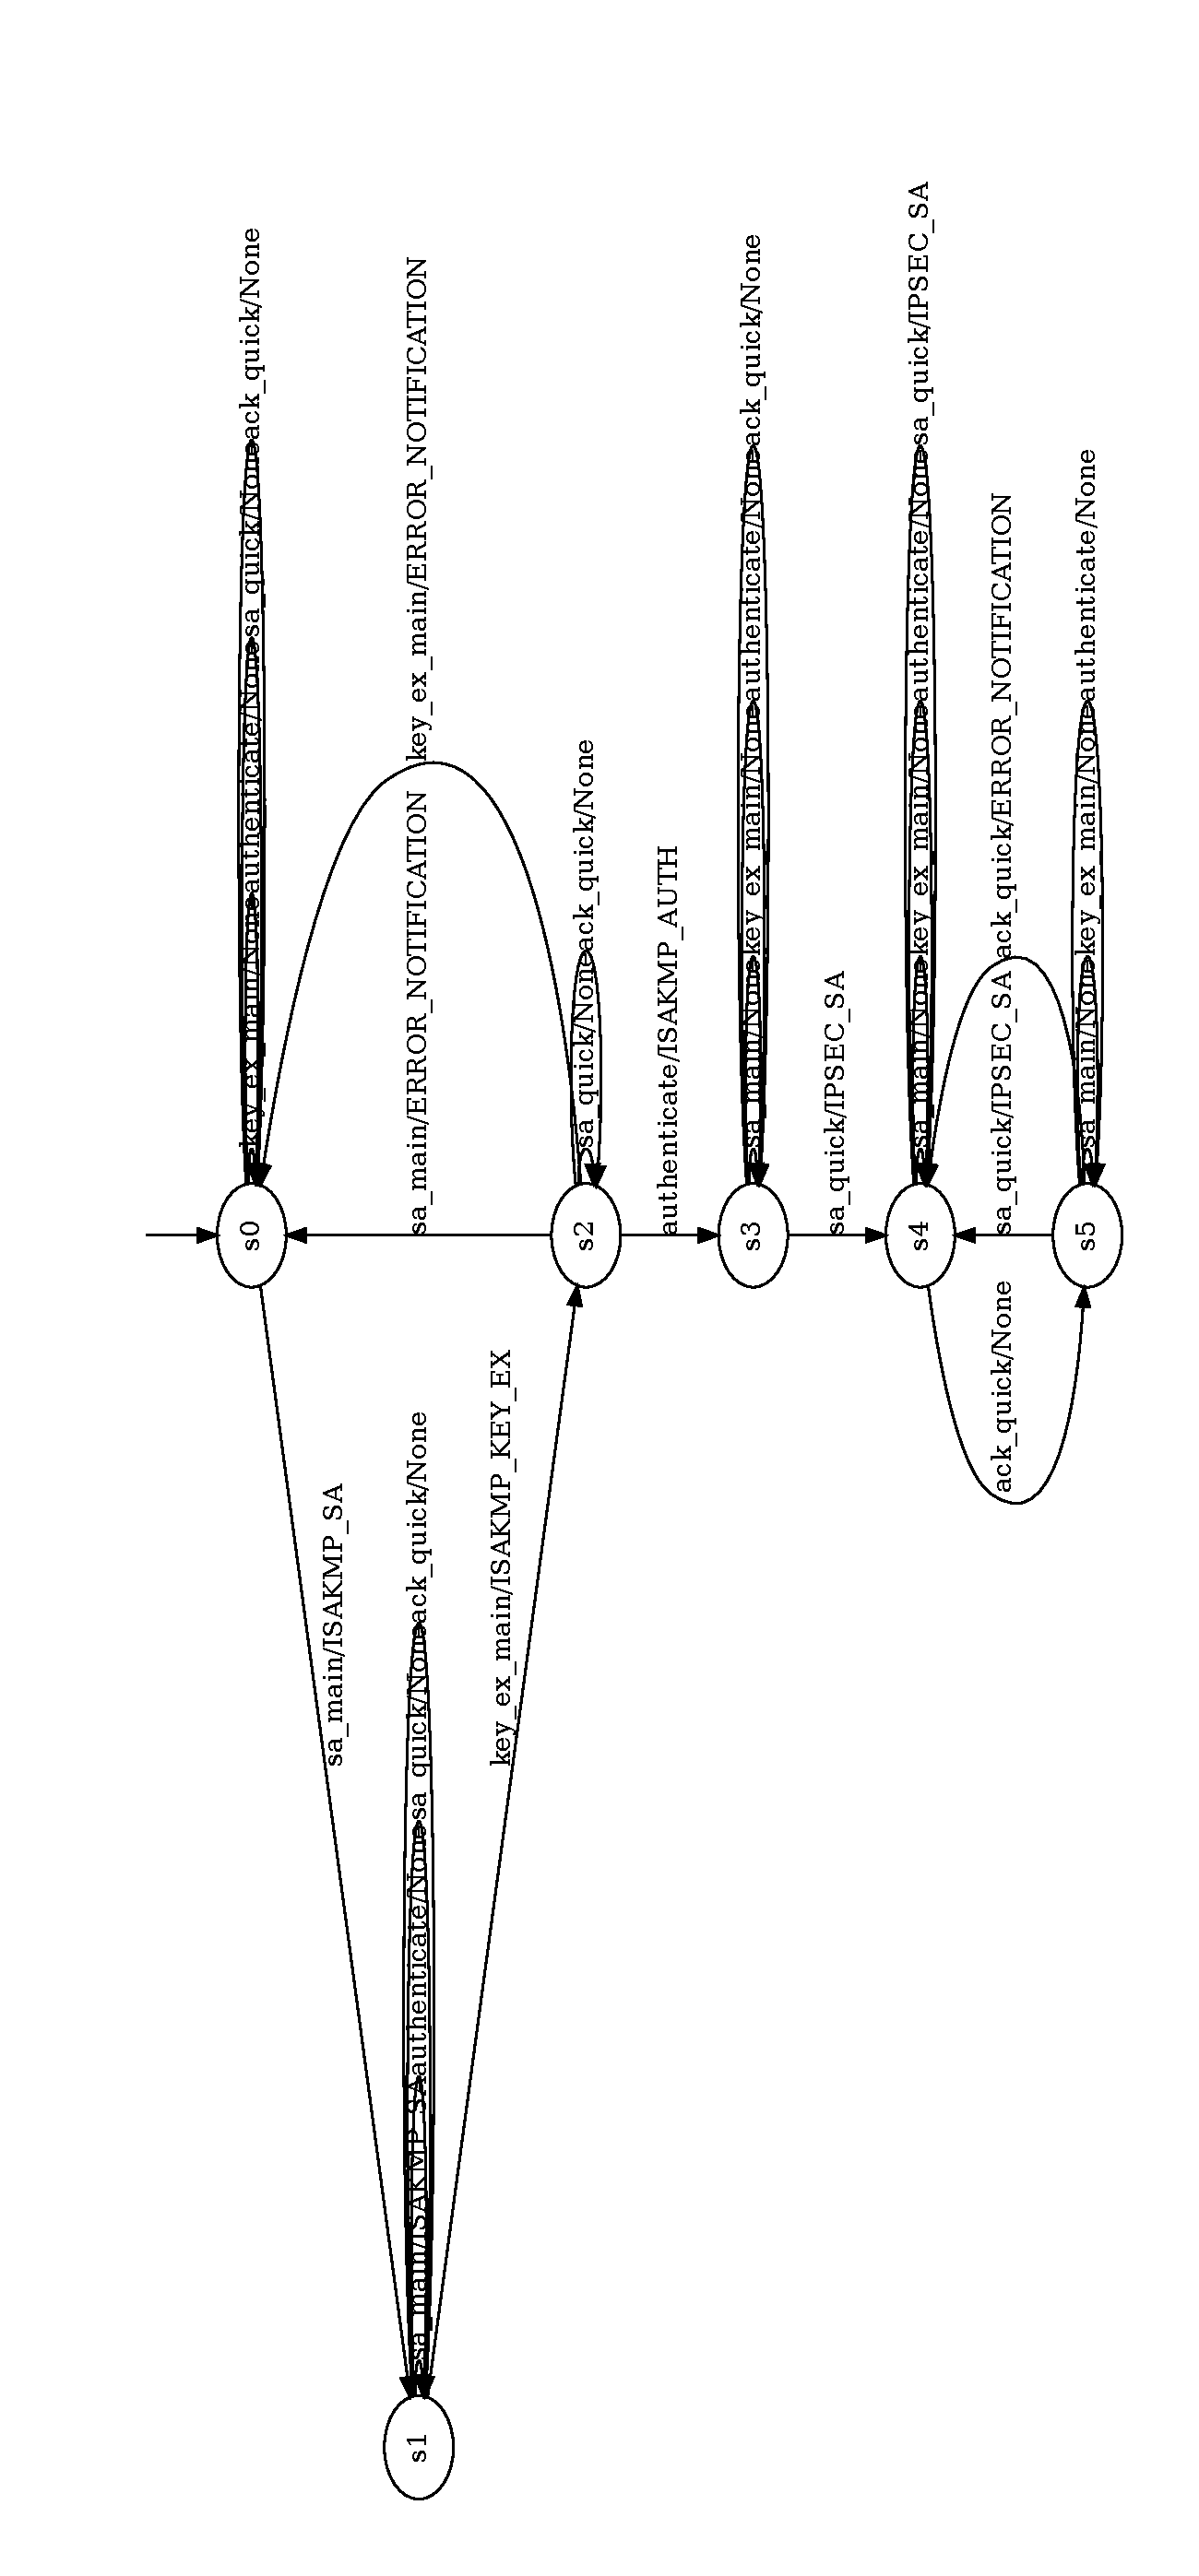
\includegraphics[width=0.7\linewidth]{images/models/Reference_rotated}
	\caption{Clean strongSwan model learned using retransmission-filtering.}
	\label{fig:reference}
\end{figure}

\subsubsection*{Fuzzing Reference Models}
% Error model
Figure \ref{fig:withfilterwitherrors} shows the (simplified, with self-transitions removed for readability) reference model used for fuzzing the strongSwan server, learned with retransmission-filtering enabled. Additionally, the input alphabet was expanded to include an additional erroneous version of each input that maps to an erroneous input. Thanks to the retransmission-filtering, the same model could be learned every time. The DOT file of the full model is provided in Appendix~\ref{app::dot}. Using the $KV$ algorithm, it took roughly 24 minutes (1447 seconds) to learn. The model took between five and four learning rounds to complete and consists of six states. Roughly 60\% of the total learning time was spent on state exploration/output queries and the remaining 40\% on conformance checking (879 vs 568 seconds). State exploration took an average of 1556 input steps to complete. In comparison, conformance checking required only 944 inputs. Alternatively, when learned using the $L^*$ algorithm, the model took a total of 51 minutes (3078 seconds) to learn over a single learning round. The 51 minutes were split between state exploration and conformance checking in a 80/20 split (2500 vs 578 seconds), with state exploration requiring 600 output queries. For this algorithm, learning took 2600 inputs and the equivalence checking required 740 input steps. Interesting to note is the large difference in conformance checking runtime between the two algorithms. For learning the reference model using $L^*$, state exploration takes up more than 80\% of the total runtime, which is the highest percentage for all the learned models, as can been seen highlighted in the runtime summary in Table \ref{tab:runtime_summary_lstar}.\\

\begin{figure}[H]
	\centering
	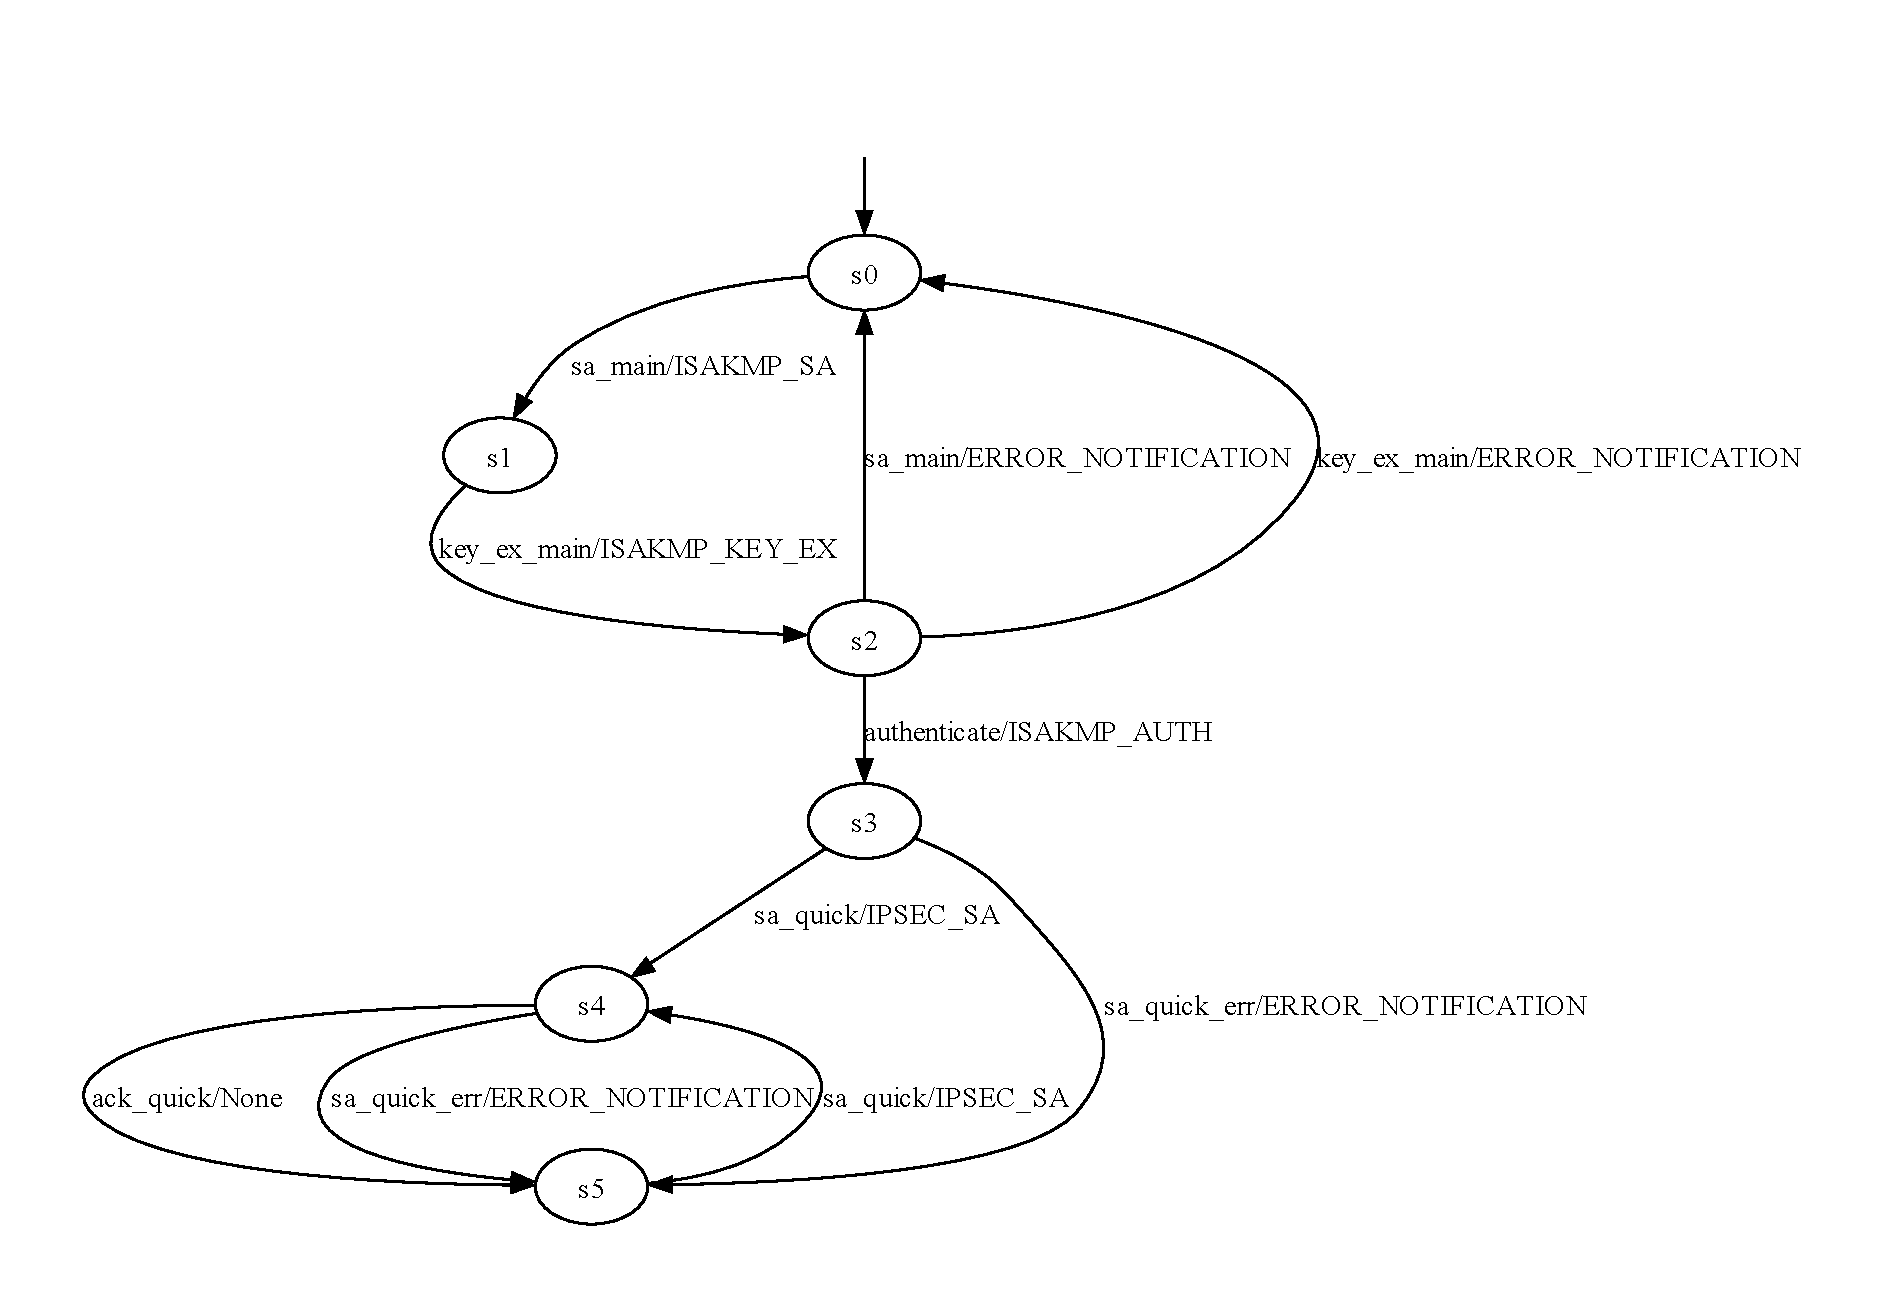
\includegraphics[width=\linewidth]{images/models/strongSwanErrKV}
	\caption{(Simplified) strongSwan model with malformed messages in the input alphabet.}
	\label{fig:withfilterwitherrors}
\end{figure}
\newpage

The model looks largely identical to the previous model, apart from some additional self and error transitions (self transitions not shown here in the simplified version). Notably, there is an error transition from state \emph{s4} to \emph{s5}, via \emph{sa\_quick\_err}. This error transition implies, that a valid \ac{ipsec} \ac{sa} is required for \emph{ack\_quick} to work. In other words, the erroneous \ac{sa} is insufficient for the server to accept an ensuing acknowledgment. If attempted, the strongSwan server returns an error message. For the same reason there is another error transition from state \emph{s3} to \emph{s5}, highlighting that one cannot complete the \ac{ipsec} handshake with invalid \ac{ipsec} \ac{sa} packets. In summation, the mentioned error transitions simply show that a valid \ac{ipsec} \ac{sa} must be created before it can be acknowledged. Note, that the DOT files of all models can be found in Appendix~\ref{app::dot} and larger PDF files of all models are available as supplementary material\footnote{\url{https://github.com/benjowun/VPN-AL}}.
\vspace{3mm}
\begin{table}[H]
	\centering
	\begin{tabular}{|l|l|l|l|l|l|l|}
		\hline
		\rowcolor[HTML]{C0C0C0} 
		Model     & States & TT (s)   & TL (s)   & TC (s)   & OQ  & CT  \\ \hline
		First Common  & 10     & 5094 & 3489 & 1605 & 462 & 100 \\ \hline
		Second Common  & 12     & 7520 & 5393 & 2126 & 522 & 120 \\ \hline
		Base      & 6      & 1652 & 899  & 753  & 177 & 60  \\ \hline
		Fuzzing Ref. & 6      & 3078 & 2500 & 578  & 600 & 60  \\ \hline
	\end{tabular}
	\caption{$L^*$ Runtimes of all the learned strongSwan models.}
	\label{tab:runtime_summary_lstar}
\end{table}
\vspace{3mm}

Table~\ref{tab:runtime_summary_averages} shows the average statistics of both learning algorithms over all four learned strongSwan models (averages of $L^*$ and $KV$ combined in one cell). As expected, models consisting of more states took longer to learn than those with less. For the two models with an identical amount of states, namely the Base and Fuzzing Reference models, the combined number of queries sent is a more suited indicator for the expected runtime. In general, the combined number of queries serves as a good indicator for how long each model will take to learn. \\
\vspace{3mm}
\begin{table}[H]
	\centering
	\begin{tabular}{|l|l|l|l|l|l|l|}
		\hline
		\rowcolor[HTML]{C0C0C0} 
		Model    	& States & TT (s)   & TL (s)   	  & TC (s)   & OQ  & CT  \\ \hline
		Common A  	& 10     & 4048 	  & 2495	 	  & 1553 	 & 317 & 100 \\ \hline
		Common B  	& 12     & 6014 	  & 3888		  & 2126 	 & 369 & 120 \\ \hline
		Base      	& 6      & 1433 	  & 690 		  & 744  	 & 128 & 60  \\ \hline
		Fuzzing Ref.& 6      & 2263 	  & 1690		  & 573  	 & 387 & 60  \\ \hline
	\end{tabular}
	\caption{Runtimes averages of both learning algorithms of all the learned strongSwan models.}
	\label{tab:runtime_summary_averages}
\end{table}
\newpage

\subsection{Learned libreswan Models}
Figure \ref{fig:learnedmodellibresimple} shows the libreswan clean base model, learned using the same input alphabet and retransmission-filtering rules. The corresponding strongSwan model is the strongSwan Base model, shown in Figure~\ref{fig:reference}. The model is very simple, consisting of only four states. Learning occurred over two rounds using the $KV$, and only one round, using the $L^*$ algorithm. Despite the aforementioned reset workaround potentially affecting runtimes and therefore them being excluded from statistics, some runtime-agnostic metrics, such as the number of required queries and steps, are still provided. Using the $KV$ algorithm, 36 output queries and 321 steps were required by the learning algorithm. Conversely, $L^*$ required 100 output queries and 350 input steps. Both algorithms required 40 conformance tests for equivalence checking, with the $KV$ algorithm however requiring roughly 660 steps, compared to the 460 of the $L^*$ algorithm. With respect to runtime, $KV$ did outperform $L^*$, but it is important to again note, that any runtime measurements for libreswan are unreliable and cannot be compared with the strongSwan runtimes, due to the reset workaround.

\begin{figure}[H]
	\centering
	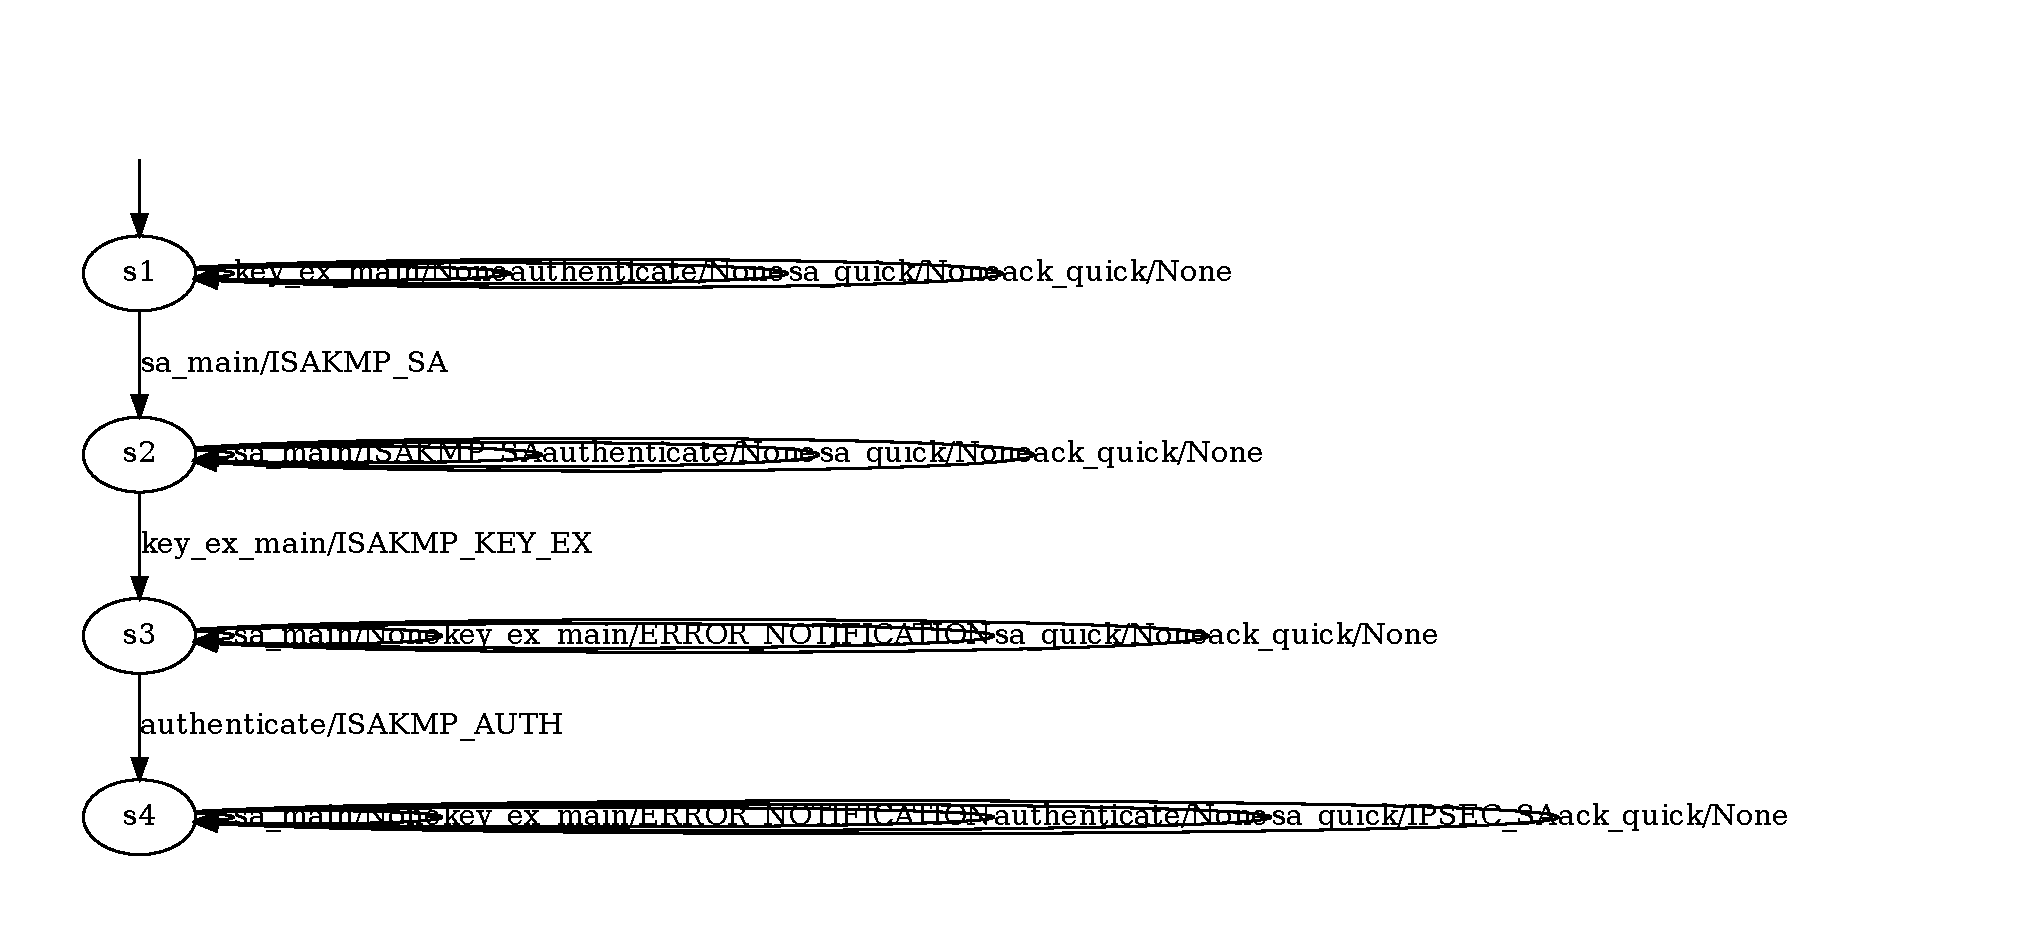
\includegraphics[width=\linewidth]{images/models/LearnedModelLibreSimple}
	\caption{Clean libreswan model learned using retransmission-filtering.}
	\label{fig:learnedmodellibresimple}
\end{figure}

The learned libreswan base model itself is noticeably smaller than its strongSwan equivalent, having two less states. In addition, the libreswan model is very linear, with each state being forced to occur subsequently. This is due to how libreswan handles errors and invalid messages, completely ignoring most error types that would lead to connection resets with strongSwan. This behavior is also what forced us to implement a workaround for the reset functionality, as error messages do not cause the libreswan phase one \ac{isakmp} connection to be closed. Another key difference is that following the initial key exchange in phase one, the libreswan server does return error messages when presented with another unencrypted key exchange request, but does not close the affected connection. In contrast, strongSwan simply ignores them in phase two resulting in a None response in the model. However, if an additional key exchange request is sent to a strongSwan server before phase one is completed, the server returns an error and aborts the connection. The key difference here being the closing of the connection on error, which again explains the more complicated strongSwan model, compared to the linear libreswan one. This difference can, e.g., be seen when comparing the transition of Figure~\ref{fig:reference}, state \emph{s2} to \emph{s0}, with state \emph{s3} of Figure~\ref{fig:learnedmodellibresimple}, noting the lack of a transition back to the initial state for the libreswan model. Finally, there is a distinct lack of error messages for not-yet established \ac{ipsec} SA acknowledgments on the libreswan server, resulting in both \emph{sa\_quick} and \emph{ack\_quick} remaining in the same state. 
\newpage


The libreswan version of the fuzzing reference model is again simpler than its strongSwan counterpart, consisting of one less state (five vs six) than the strongSwan fuzzing reference model. The DOT file of the full automata can be found in Appendix~\ref{app::dot}. Figure~\ref{fig:learnedmodellibrereference} shows a strongly simplified model, without self-transitions, highlighting the new state \emph{s2}. It looks largely identical to the libreswan base model, with the notable addition of a left branch in the model (state \emph{s1} to \emph{s2}), where an erroneous \emph{sa\_main\_err} packet is sent at the start of the connection. This causes the server to become impossible to establish a connection with (with our setup), as libreswan ignores any further attempts with the same initiator cookie, following an invalid one, regardless of their correctness. The server does not leave this error state any more, as due to the \emph{uniqids} setting mentioned in Chapter~\ref{chap:Setup}, all following \emph{ISAKMP\_SA} packets will use the same ID. While the admittedly a rather uncommon server setup (primarily used here due to simplify our mapper class), it could be considered a design flaw, to block valid \emph{ISAKMP\_SA} packets from replacing a broken connection when using the \emph{uniqids} setting, as this renders the connection unusable. A valid use-case for this setting could be wanting to connect multiple users using a single \ac{ike} connection.

\begin{figure}[H]
	\centering
	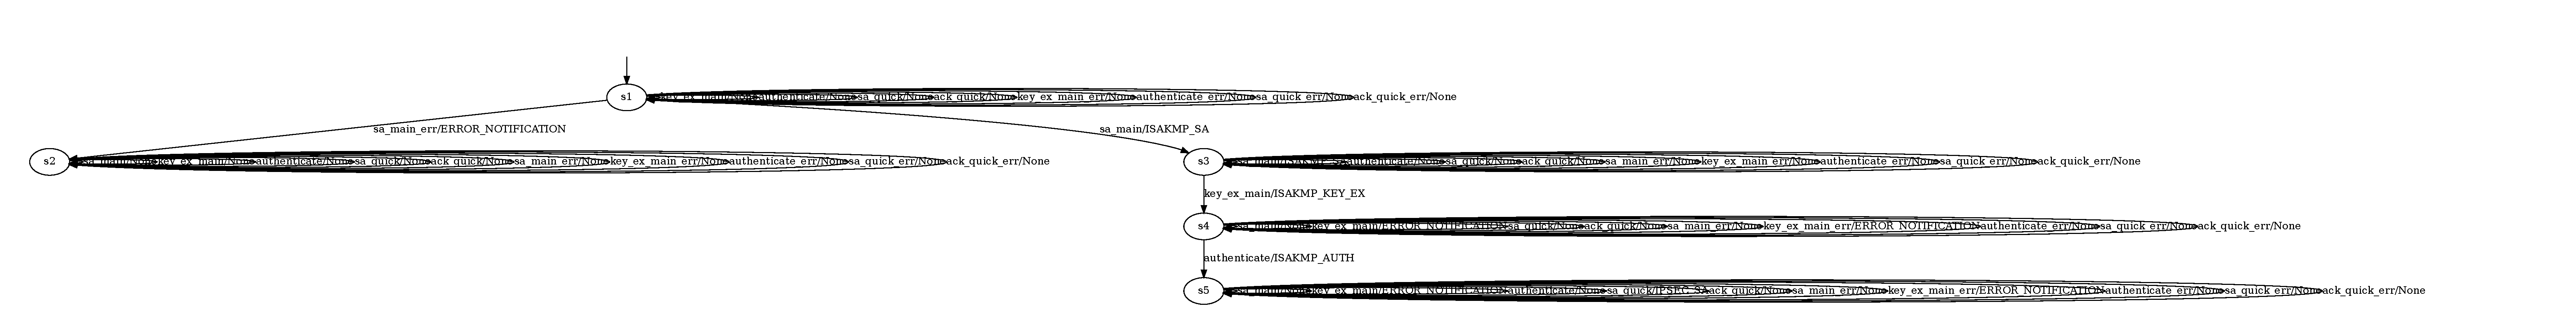
\includegraphics[width=0.7\linewidth]{images/models/LearnedModelLibreReference}
	\caption{(Simplified) libreswan model with malformed messages in the input alphabet.}
	\label{fig:learnedmodellibrereference}
\end{figure}

As switching to a randomly generated initiator cookies system would have negatively affected the strongSwan setup, the decision was made against a random-initiator cookie redesign. Especially since the libreswan setup already required a workaround for its reset method, potentially skewing results, the additional reworks were considered not worth the effort, but should be considered for future work.\\

In summation, one can say that the strongSwan server is stricter with their error handling, closing connections if errors are encountered, whereas libreswan is more error-tolerant, preferring to keep connections regardless. These implementation details are clearly visible in the presented models, with the libreswan model having considerably less states, due to less error-handling being performed.
\newpage

\subsection{Comparing $KV$ and $L^*$} \label{subsec:comp_kv_lstar}
% section copmaring KV and Lstar
Table \ref{tab:compkvlstar} shows average performance statistics over 20 learning attempts for both learning algorithms on the strongSwan server. The models were learned with retransmission-filtering enabled. The same hardware and software configurations were used as described in Chapter~\ref{chap:Setup} with the learning program set up on a VirtualBox 6.1 \ac{vm} allotted 4GB of memory and one CPU core. We used all the basic packets for our input alphabet, so
\emph{sa\_main}, \emph{key\_ex\_main}, \emph{authenticate}, \emph{sa\_quick} and \emph{ack\_quick}. The model learned is the clean model seen in Figure \ref{fig:reference}. Table~\ref{tab:compkvlstar} shows the metric on the left and the respective averages for the $L^*$ and $KV$ learning algorithms respectively on the right. Interesting results are highlighted in bold. From top to bottom, the metrics measured are as follows. Learning rounds refers to the number of rounds the learning algorithms had to run for, or in other words, how many hypotheses they needed to propose to the teacher in order to correctly learn the \ac{sul}. Total time is the total time needed by the algorithm from start to the finished model. The total time can be split into time spent on the state exploration and time spent on equivalence queries. Learning output queries refers to the number of output queries sent to the SUL while learning steps to the number of individual inputs executed on the \ac{sut}. Analogously, equivalence oracle queries refers to the equivalence queries sent to the SUL and equivalence oracle steps to the inputs executed by the equivalence oracle. Finally, output queries saved by caching details the performance boost gained by caching output queries, with the value indicating the number of queries saved.

\begin{table}[h]
	\centering
	\begin{tabular}{ |p{6.5cm}||p{1cm}|p{1cm}|  }
		\hline
		\multicolumn{3}{|c|}{\textbf{Learning Algorithm Performance (Averages)}} \\
		\hline
		\textbf{Metric} & $\mathbf{L^*}$ & $\mathbf{KV}$ \\
		\hline
		Learning Rounds							&	2				&	4 				\\
		Total Time (s)							&   1652			& 	1214   			\\
		Time Learning Algorithm	(s)				&	\textbf{899}	& 	\textbf{480}	\\
		Time Equivalence Checks (s)				& 	753				& 	734			\\
		Learning Output Queries 				&   \textbf{177}	& 	\textbf{78}		\\
		Learning Steps							& 	856	  			& 	676   			\\
		Equivalence Oracle Queries				& 	60  			&  	60				\\
		Equivalence Oracle Steps				& 	747  			&  	934				\\
		Output Queries Saved by Caching			& 	\textbf{13}		&  	\textbf{30}				\\
		\hline
	\end{tabular}
	\caption{Comparison of the $L^*$ and $KV$ learning algorithms.}
	\label{tab:compkvlstar}
\end{table}

As the only difference between the two configurations tested was the choice of learning algorithm, intuitively one expects relevant fields to vary the most with equivalence oracle field to be largely unchanged. This intuition is confirmed by our experiments, wherein while the time spent on equivalence queries was very similar, with both requiring the same number of equivalence oracle queries for conformance checking. In contrast, the time spent on output queries differs greatly between the two model-learning algorithms. The $L^*$ algorithm required almost double the number of output queries than its $KV$ counterpart. As communication with the \ac{sut} is the main performance bottleneck and output queries make up a large portion of this communication, this change naturally led to a significantly better runtime for $KV$, with total time spent on the learning algorithm being close to half that of the $L^*$ algorithm. This difference in time spent on the learning algorithm meant, that for this experiment, the $KV$ algorithm learned a model in roughly 75\% of the time needed by the $L^*$ algorithm. Looking only at the learning algorithm, $KV$ performed roughly twice as well as its counterpart. As the same equivalence checking algorithm was used for both attempts, the identical number of equivalence oracle queries makes sense. Another noticeable difference can be observed in the number of output queries saved by caching. Here, $KV$ saves more than double the amount $L^*$ does, indicating a better caching implementation. In summation, we found the $KV$ algorithm to be better suited for our learning setup and solely used it for fuzzing. \\\\

Little variance was observed throughout all learning attempts so the sample size of 20 learning attempts each is believed to be representative. However, for even more accurate results the experiment should be carried out again for even more input sequences. Additionally, it might be interesting to compare the performance of various equivalence oracles for this learning setup.

\subsection{Library Error} \label{subsec:liberror}
% section with discovered bug
Another notable finding from the model learning phase, which demonstrates the usefulness of \ac{aal} from a testing standpoint, was the discovery of a bug in a used Python Diffie-Hellman key exchange library. The bug was only found thanks to the exhaustive number of packets sent with our mapper class and due to the non-determinism checks implemented in \textsc{AALpy}. Despite our best efforts in removing the non-deterministic behavior from our learning process, we would still get occasional non-determinism errors at random points while learning. This problem persisted over several weeks due to the fact that the errors occurred randomly and only sporadically during some learning attempts. Initially we believed this to be also caused by retransmissions, but since the problems persisted even after introducing retransmission-filtering, that possibility was ruled out. The other option was of course problems in our implementation of the \ac{ipsec} protocol. Therefore, a lot of time was invested into painstakingly comparing logs and packet captures between our implementation and the \ac{sul} to ensure that everything lined up, since \textsc{AALpy} was still reporting non-determinism errors. Finally, a small discrepancy between the two logs was discovered and through it, that the problems were not in fact caused by our implementation, but by a used Python library. It turns out there was a very niche bug in a used Diffie-Hellman Python library~\cite{topdappdh}, where if the \ac{msb} was a zero, it would be omitted from the response, causing the local result to be one byte shorter than the value calculated by the \ac{sul}. As this would only occur in the rare case where the \ac{msb} of the DH exchange was zero, this explains the random and difficult to reproduce nature of the bug. This behavior was undocumented and happened in a function call that allowed specifying the length of the returned key. As the library is not a very widespread one, the impact of this bug is presumably not very high. Regardless, it could compromise the security of affected systems and therefore the maintainer of the library has been notified of the problem. Due to the elusive nature of this bug, it would very likely not have been noticed without the exhaustive communication done by the model-learning process and without seeing the slight differences in the resulting models that did not crash during the learning process.
\newpage

\section{Fuzzing Results} \label{sec:fuzzresults}
We used model-based fuzzing to test the two \ac{ipsec} \ac{ike}v1 \acp{sut}. Our fuzzer supports testing inputs in the context of input sequences, to ensure an identical state on the \ac{sut} for each fuzzed input. To that end, we developed a custom fuzzer supporting multiple methods of generating the input sequences to be tested, filtering, search and genetic algorithm-based input-sequence generation, as described in Chapter~\ref{chap:Fuzzing}. All fuzzing took place in the same isolated network described in Chapter~\ref{chap:Setup}. The used fuzzing reference models can be seen above in figures \ref{fig:reference} and \ref{fig:learnedmodellibrereference}, for strongSwan and libreswan respectively. This section presents the results of using our custom fuzzer to fuzz both a strongSwan, as well as a libreswan \ac{ipsec} server. Different input-sequence generation methods were used and contrasted, comparing performance and discovered findings. Most methods found the same issues, however the search-based input-sequence generation method proved to be the fastest and the genetic method resulted in the best fitness score. Randomly generated input sequences serving as a baseline did not discover all the findings. \\

\subsection{Findings} \label{subsec:findings}
Our fuzzer was very successful in discovering new behavior not covered by the reference model, finding new cases for almost every input sequence tested with both input-sequence generation methods. As discovered new behavior does not necessarily indicate that the new behavior is harmful, the discovered new transitions still had to be manually parsed for particularly interesting behavior. By analyzing the specific concrete inputs leading to new transitions, we discovered two undocumented instances of the \ac{sut} not following RFC specifications. Unfortunately, a lot of ``non-findings'' were discovered as well, with non-findings referring to new behavior not covered by the reference model, but also not exhibiting undocumented or otherwise interesting behavior. Some of these non-findings could be removed by simply specifying some fields which should not be fuzzed. Unfortunately, this approach requires manually going through and verifying that none of the discovered behavior is interesting. Alternatively, it might be possible to use the discovered new behavior to generate a suite of tests checking for common exploitable vulnerabilities, such as buffer overflows and memory leaks. However, this goes beyond the scope of this thesis.

To further reduce the amount of information that had to be manually reviewed, we improved the fuzzer by temporarily adding newly learned states and transitions to the reference model as soon as they are discovered. This stops the fuzzer from repeatedly discovering the same new behavior with different variations of the same fuzzed input, leading to far less manual reviewing being required. For completeness sake, we first present some of the more interesting or common non-findings, followed by the two discovered deviations from the RFC specifications. Unless otherwise mentioned, all findings were found on both tested \ac{ipsec} servers.

An example of a non-finding that is typically categorized as noise is the discovery of new behavior by changing the initiator/responder cookies as part of fuzzing. These cookies are used in part to identify the members of a \ac{vpn} connection. The new behavior was detected, as during the learning of the reference model, the cookies were not changed mid-input sequence execution, as this causes the \ac{sut} to think it is communicating with a different user and if it doesn't know that user, to simply discard the message. As fuzzing the cookie fields did not lead to any errors on the server side and greatly complicated the mapper class, this field was removed from the fuzzing scope. 

Another non-finding was discovered while fuzzing the field indicating the number of proposals in the \emph{ISAKMP SA} packet. While testing various randomly chosen lengths, every time the length was set to one, the fuzzer indicated, that a new state had been found. This behavior was caused due to our implementation of both the fuzzer and base reference model. Our \emph{ISAKMP SA} packet always contains exactly one proposal and the packet being fuzzed is assumed to be incorrect. However, in this case, the field is, by fuzzing through random numbers, every so often set to a valid value (namely one), resulting in a mismatch between the expected (error) and actual (normal) response. 
Yet another cause of many non-findings during fuzzing were the various packets containing hashes, e.g., \emph{ACK} and \emph{AUTH}. Fuzzing these hashes proved to be problematic, as random changes to the hashes causes the server response encryption to no longer match the mapper class, making decryption impossible. Therefore, errors had to be manually examined in the strongSwan logs. Seeing as no crashes or other unexpected errors were observed, fuzzing hashes was reduced in the overall fuzzer. 

Overall, while examining and testing the discovered new behavior helped improve our overall understanding of the \ac{ipsec} protocol, it rarely resulted in the discovery of any actual undefined/undocumented behavior. However, in two separate cases, actual deviations from the relevant RFC specifications were observed with the \acp{sut}. \\

The first of these deviations was discovered while fuzzing the \ac{isakmp} header length field. This field is specified by RFC 2409~\cite{rfc:isakmp} (\ac{isakmp} protocol definition), as the length of the entire \ac{isakmp} packet. When manually going through the results of the fuzzer, a significant amount of the newly discovered behavior was found to have been caused by packets with a fuzzed \ac{isakmp} header length field. Comparing the responses to the fuzzed packets revealed, that they did not match the expected return values according to the reference model. As expected and actual return values did not conform, the fuzzer correctly concluded, that a new state had been found. The mismatch between actual and expected values was caused by the reference model expecting an error response to the fuzzed \ac{isakmp} length field, while in practice, both of the tested \acp{sut} ignored the content of the field entirely. This behavior is showcased in Listing~\ref{lst:finding_isalen}, Line~\ref{line:finding_isalen_1}, where an error was expected, but the \ac{sut} returned a valid response, despite the length field having the obviously incorrect value of hex $FF000000_{16}$ ($4278190080_{10}$). The finding was similarly observed with all other tested values, in all ranges from zero to $FFFFFFFF_{16}$, leading us to the conclusion that the field is in fact completely ignored by both \ac{ipsec} servers. \\
\vspace{3mm}
\begin{lstlisting}[float=h, caption=Discovered finding showing the ISAKMP length field being ignored., label=lst:finding_isalen, escapechar=§]
	Fuzzing isa_len with: b'\xff\x00\x00\x00'
	Input sequence: ['sa_main_fuzz', 'key_ex_main', 'authenticate', ...]
	$sa_main_fuzz

	**********
	Expected: ERROR_NOTIFICATION | Received: ISAKMP_SA §\label{line:finding_isalen_1}§
	**********
	
	$key_ex_main
	**********
	Expected: None | Received: ISAKMP_KEY_EX
	**********
	
	$authenticate
	**********
	Expected: None | Received: ISAKMP_AUTH
	**********
	...
\end{lstlisting}
\newpage
The impact of this finding is presumably rather small, however it might lead to inconsistencies between different \ac{ipsec} implementations, should they handle this behavior differently. Additionally, RFC 2048 (describing \ac{isakmp}) clearly specifies, that the \ac{isakmp} payload length field must match the length of the entire payload. Seeing as \ac{ipsec} heavily relies on \ac{isakmp}, these requirements should still hold true. This is especially relevant, as strongSwan even lists RFC 2408 as one of the ``Core Standards'' they adhere to on their own website~\cite{strongswan-ietf}. In fact, RFC 2409 (IKEv1), Section 5~\cite{rfc:ikev1} states very plainly, that \ac{ike}v1 exchanges are to conform to the \ac{isakmp} standard.
This standard, in Section 5.1 of RFC 2048~\cite{rfc:isakmp} states the following. 

\begin{quotation}
	``...If the ISAKMP message length and the value in
	the Payload Length field of the ISAKMP Header are not the same, then
	the ISAKMP message MUST be rejected.''
\end{quotation}

In other words, according to the RFC, the length field-manipulated \ac{isakmp} packets are invalid and should be rejected. Since the tested strongSwan and libreswan servers do not, this finding falls into the deviations from specifications category.  \\

Another interesting finding can be observed on strongSwan servers when fuzzing the transform \texttt{Authentication} field sent at the start of an \ac{ike} exchange as part of an \emph{ISAKMP SA} packet. The expected behavior for the fuzzed field was, that the server would return an error response right away, indicating it does not support the proposed unknown \texttt{Authentication} method. However, in practice, the error response was only received from the tested strongSwan server after the key exchange packet was sent as well. strongSwan logs also do not show any errors when parsing in an \emph{ISAKMP SA} packet with a fuzzed \texttt{Authentication} transform field. This is due to strongSwan apparently only verifying the content of the \texttt{Authentication} transform field during the key-exchange step. Listing~\ref{lst:finding_auth} shows the results of fuzzing the strongSwan \ac{sut} using a modified unsupported \ac{isakmp}\_SA \texttt{Authentication} transform field. \\
\vspace{3mm}

\begin{lstlisting}[float=h, caption=Discovered finding showing the Authentication field not being validated., label=lst:finding_auth, escapechar=§]
	Fuzzing tf with: [('Encryption', 'AES-CBC'), ('KeyLength', 256), ('Hash', 'SHA'), ('GroupDesc', '1024MODPgr'), ('Authentication', '65535'), ('LifeType', 'Seconds'), ('LifeDuration', 28800)]
	
	Run: ['sa_quick_err', 'ack_quick', 'sa_main_fuzz', 'sa_quick_err', 'authenticate_err', 'sa_quick_err', 'key_ex_main', 'authenticate', 'sa_main', 'key_ex_main']
	
	$sa_main_fuzz

	**********
	Expected: ERROR_NOTIFICATION | Received: ISAKMP_SA §\label{line:finding_auth_1}§
	**********
\end{lstlisting}

\newpage
Listing~\ref{lst:finding_auth}, Line~\ref{line:finding_auth_1} shows, that the \ac{sut} does not return an error and instead returns a valid \emph{ISAKMP SA} response packet. This is problematic, as RFC 2049, section 5~\cite{rfc:ikev1} explicitly states that 

\begin{quotation}
	``Exchanges conform to standard ISAKMP payload syntax, attribute
	encoding, timeouts and retransmits of messages, and informational
	messages-- e.g a notify response is sent when, for example, a
	proposal is unacceptable, or a signature verification or decryption
	was unsuccessful, etc.''
\end{quotation}

In particular the second part regarding a notification being sent for unacceptable proposals leads us to believe, that the behavior exhibited by the strongSwan \texttt{Authentication} transform field is unintended behavior, that deviates from the RFC specification. It is important to note, that only the \texttt{Authentication} field exhibited this behavior, all the other tested transform fields (\texttt{Encryption}, \texttt{KeyLength}, \texttt{Hash}, \texttt{Group Description}, \texttt{Life Type} and \texttt{Life Duration}) appear to be checked right away and return errors if invalid/unknown. This further supports the theory, that validity checks for this particular field were simply forgotten. Another interesting point to note is that Wireshark logs of the sent packets show, that the response transform has the \texttt{Authentication} field set to \ac{psk}, despite the fuzzed value sent to it not being supported. This indicates, that for this field strongSwan reverts to a default value if it encounters an invalid input, without logging any errors. This is problematic in its own right, as errors being belatedly reported makes debugging more difficult. The main impact of this finding is therefore most likely its potential in making debugging more difficult. It is important to highlight, that this finding was only observed on the strongSwan server, the libreswan server seems to implement it correctly. \\

While not necessarily severe findings, the two RFC specification deviations clearly do not conform to \ac{isakmp} and \ac{ipsec} standards. As deviations from specifications can lead to vulnerabilities and compatibility issues, they should be carefully reviewed to ensure that they are intentional and not due to an oversight. In particular the \texttt{Authentication} field finding should be checked, as all other fields of that packet exhibited the correct behavior, indicating a potential developer oversight. It is important to thoroughly examine any deviations from established standards to ensure that the system is as secure as possible. \\

Finally, reviewing the learned libreswan model in Figure~\ref{fig:learnedmodellibrereference} revealed a potential deadlock state, state \emph{s2}. The learned model suggests, that the libreswan \ac{ipsec} server does not recover from an invalid initial \emph{\ac{isakmp} SA} packet. Further testing showed this to be accurate, with all packets being ignored following the initial erroneous one. While likely limited to our particular \ac{ipsec} configuration, notably the \emph{uniqueids} setting allowing us to reuse the existing connection, this could prove problematic in certain edge cases, where IDs are not unique and due to network errors, the first packet is invalid. In such a scenario, the connection would remain unusable until the server is restarted. This problem does not occur with the strongSwan implementation, as strongSwan destroys the \ac{isakmp} connection when an erroneous packet is received prior to keying.
\newpage
\subsection{Comparison of Input-Sequence Generation Methods} \label{subsec:mutation_vs_filtering}
This subsection compares the performance of the utilized input-sequence generation methods used for fuzzing. The methods are filtering, search and genetic algorithm-based input-sequence generation approaches and are explained in detail in Chapter~\ref{chap:Fuzzing}. Additionally, random input sequences were used to serve as a baseline when comparing the other input-sequence generation methods. All methods other than the random baseline led to input sequences that discovered all above-mentioned non-trivial findings during fuzzing. However, the methods differ greatly with regards to the amount of coverage achieved and their runtime. \\

As the filtering-based input-sequence generation method results in many different input sequences, that are then all fuzzed, naturally its coverage is inherently higher the other methods, which result in only a single (or a select few) input sequence(s). This is due to the filtering-based approach reusing the input sequences already generated during model learning of the fuzzing reference model, bringing with it a guarantee of state-coverage (for at least the reference model). While this guarantee does not necessarily still hold after removing some input sequences due to filtering, considering the large number of remaining ones, the resulting coverage after fuzzing all of them will almost certainly be significantly higher than when limited to one, or very few, input sequences. However, as a trade-off, the runtime of fuzzing the input sequences generated through the filtering-based method is exceedingly long, as can be seen in Table~\ref{tab:compfuzz}. The runtime of the filtering step itself is less than the other methods, as seen in Table~\ref{tab:comprun}, and also more consistent, as the duration of the filtering algorithm is less random than that of the search or genetic-based methods. However, the fuzzing runtime is far longer than that of the other methods, as all the remaining input sequences are fuzzed one after the other. This leads to the fuzzing runtime of the filtering-based approach being more easily measurable in days instead of hours. Unfortunately, due to the extremely long runtime and our limited resources, this method could only be used sparingly, making the resulting statistics less tested than the others. 

\vspace{3mm}
\begin{table}[H]
	\centering
	\begin{tabular}{|l|l|}
		\hline
		\rowcolor[HTML]{EFEFEF} 
		\textbf{Method} & \textbf{Runtime (h)}   \\ \hline
		Filtering		            &  7	     \\ \hline
		Search              		&  19.5      \\ \hline
		Genetic              		&  15.6       \\ \hline
	\end{tabular}
	\caption{Comparison of input sequence generation runtimes using the strongSwan server.}
	\label{tab:comprun}
\end{table}

In comparison, the search-based input-sequence generation method results in only a single input sequence to be fuzzed, albeit one that is then fuzzed in more detail (all inputs of the sequence instead of only one are fuzzed). Using the search-based approach described in Chapter~\ref{chap:Fuzzing}, a single input sequence is continuously refined with regards to a fitness score. The fitness score describes the suitability of the input sequence in finding new behavior, as well as achieving a high degree of state-coverage when fuzzed. Table~\ref{tab:compbasesearch} shows a comparison of our generated and random baseline input sequences, examining their average fitness scores with regards to the strongSwan server. Two baseline sequence lengths were used as a comparison, one consisting of eight inputs and the other out of 18. These lengths mirror the lengths of the best-scoring input sequences generated through search/genetic-based methods. The fitness score for the filtering method was calculated by calculating the average fitness score of all the input sequences produced by the filtering method. While considerably more performative than both baseline sequences, the filtered input sequence fitness score is barely half as good as that of the search-based method. Comparing search with the two baseline sequences shows that it significantly outperforms both. The poor results of the baseline sequences can be explained by the baseline fuzzing often getting stuck in the initial state/phase and therefore lacking coverage of large parts of the \ac{sut}. This naturally leads to a poor score, as hardly any interesting behavior is found and the coverage is poor. As both of the discovered findings were discoverable in the initial state however, no concrete differences in the actual discovered findings were observed for that state. However, fuzzing the baseline sequences resulted in far fewer findings, especially the \ac{isakmp} length finding, as far fewer states were covered. The filtering method does discover all findings, however the fuzzing runtime is disproportionately longer, as shown in Table~\ref{tab:compfuzz}. Additionally, while the average runtime of the search-based method is inferior to the filtering-based method, see Table~\ref{tab:comprun}, the actual fuzzing is considerably quicker, making the total runtime (sequence generation + fuzzing) also quicker. Consequently we argue, that the search-based method significantly outperforms both the baseline and filtering-based methods, making it more likely to discover interesting behavior while fuzzing, in less time, even if no additional findings were found for the specific \acp{sut} in question. 

\vspace{3mm}
\begin{table}[H]
	\centering
	\begin{tabular}{|l|l|}
		\hline
		\rowcolor[HTML]{EFEFEF} 
		\textbf{Method} & \textbf{Fitness Score}  \\ \hline
		Baseline (8)              	&  0.0542     \\ \hline
		Baseline (18)              	&  0.392      \\ \hline
		Filtering (avg)             &  1.4712     \\ \hline
		Search              		&  2.8125     \\ \hline
		Genetic              		&  4.7        \\ \hline
	\end{tabular}
	\caption{Comparison of the fitness scores of input-sequence generation methods.}
	\label{tab:compbasesearch}
\end{table}

While a good trade-off in terms of time and fitness score, the effectiveness of the search-based method can be further enhanced by incorporating genetic algorithm components. As described in Chapter~\ref{chap:Fuzzing}, our genetic input-sequence generation method works similarly to the search-based approach, however, instead of mutating only one input sequence, multiple sequences called populations are mutated simultaneously. The top scoring populations with regard to the fitness function are then crossed to create new sequences with characteristics of both parent sequences. Combined with randomly generated sequences to introduce more variability, this method outperforms all other implemented input-sequence generation methods significantly, as can be seen in Table~\ref{tab:compbasesearch}. The genetic algorithm-based input-sequence generation method was configured to resemble the search-based approach with regard to the number of mutations performed on the populations. Regardless, the genetic method outperformed both the search-based and filtering-based approaches, generating an input sequence with almost double the fitness score than that of the search-based sequence, and more than thrice the score than that of the average filtering-based sequence, with similar average runtimes to the search-based approach. Note, that the runtimes for search and especially genetic algorithm-based methods have a rather high variance, as the runtime is strongly tied to the length of input sequence, which is to a certain degree, random. Furthermore, the genetic algorithm introduces populations of a random length, often significantly shorter than the current average, whereas the search-based method input sequence tends to only grow longer as it progresses. As many of the scored sequences of the genetic algorithm-based approach were short/mostly invalid due to their random generation, less inputs were actually executed on the \ac{sut}. These two attributes led to the genetic algorithm runtime being, on average, slightly better than the search-based method, however the standard deviation was significantly higher. Additionally, fuzzing the search-based and the genetic input sequences both discovered all known findings, however, the genetic sequences provided better state coverage of the reference automaton, further cementing it as an improvement over the single-population search-based method.
\newpage

Table~\ref{tab:compfuzz} shows the fuzzing runtime comparison of fuzzing the previously generated input sequences on the strongSwan \ac{sut}. The search-based method was set to run for 50 iterations and the genetic algorithm-based method was configured to use ten populations and to run for five iterations (totaling the same 50 iterations for both methods). The filtering-based approach used the input sequences from learning the reference model of the strongSwan \ac{sut} and all runtime data was measured using the strongSwan setup. The ``Fuzzed In.~Seq.''~row refers to the number of input sequences generated by the method in question that are then fuzzed. Note, that while the genetic algorithm-based input-sequence generation method technically generates several input sequences in a population, only the best-scoring sequence was fuzzed. The ``In.~Seq.~Length'' row indicates the average amount of inputs per run. The ``Seconds/In.~Seq.''~row displays the average execution time of a single input sequence and the ``Values Tested'' row shows the total number of fuzzed values tested during fuzzing rounded to the nearest hundred. Finally, the ``Runtime'' row indicates the total runtime of fuzzing the input sequence(s) in question. These metrics allow for a comparison of the efficiency and effectiveness of the two methods in generating and testing input data.


\begin{table}[H]
	\centering
	\begin{tabular}{|l|l|l|l|}
		\hline
		\rowcolor[HTML]{EFEFEF} 
		& \textbf{Filtering}					& \textbf{Search} 			& \textbf{Genetic}  \\ \hline
		\textbf{Fuzzed In. Seq.}            	& 55                 					& 1                			& 1					\\ \hline
		\textbf{In. Seq. Length}				& 14                					& 8               			& 18		  		\\ \hline
		\textbf{Seconds/In. Seq.}     			& 14                					& 8                			& 18				\\ \hline
		\textbf{Values Tested}     				& 192500              					& 2800		    			& 4500				\\ \hline
		\textbf{Runtime (h) Fuzzing}       		& 53          	 						& 7          				& 24				\\ \hline
	\end{tabular}
	\caption{Comparison of generated input-sequence fuzzing runtimes on the strongSwan server.}
	\label{tab:compfuzz}
\end{table}

Examining the strongSwan fuzzing runtime statistics shown in Table~\ref{tab:compfuzz}, the most striking difference is the difference in number of input sequences fuzzed. While the filtering input-sequence generation method resulted in 55 input sequences, the other two methods only result in one sequence. Naturally, as all 55 sequences are then fuzzed, the fuzzing runtime is by far the longest for this method. This is despite the fact that for the filtering input sequences, only one input is fuzzed, while for the other two methods, all inputs are fuzzed. \\

Each additional input added to an input sequence leads to, on average, an additional second of runtime when executing the sequence, due to timed waits and timeouts during network communication. Therefore ``In.Seq Length'' translates directly to the  ``Seconds/In.Seq.'' metric. When fuzzing, we execute the entire sequence for each value inserted into the field being fuzzed. Consequently, the total runtime when fuzzing an input sequence can be approximated as the length of the sequence (the number of inputs), multiplied by the number of values tested while fuzzing the sequence. The average number of tested values on a single input is approximately 250 values. This lets us approximate the runtime of fuzzing an input sequence as

\begin{equation}
	r = l \cdot n \cdot v
\end{equation}
\vspace{3mm}

where $l$ is the length or average length of the tested input sequence(s), $n$ the number of input sequences to be fuzzed and $v$ the average number of values tested when fuzzing one input, so 250. Consequently, we can say the runtime of our fuzzer is directly proportionate to the number of fuzzed input sequences and the length of the tested input sequence(s). There is some variance with $v$ depending on the type of tested fields, but in our case it is mostly constant. 
\newpage
Finally, Table~\ref{tab:compfull} shows the full runtimes for all used input-sequence generation methods. We can again clearly see, that despite having the shortest generation runtime, the exceedingly long fuzzing runtime makes the filtering-based approach by far the slowest. The search-based method finishes in less than half the time needed by the filtering-based approach, and discovered the same findings. However, its state coverage was less. In contrast, the genetic algorithm-based approach ran slightly longer than the search-based one, but still much faster than the filtering-based approach and had better coverage than the search-based approach.

\vspace{5mm}
\begin{table}[h]
	\centering
	\begin{tabular}{|l|l|}
		\hline
		\rowcolor[HTML]{EFEFEF} 
		\textbf{Method} & \textbf{Runtime (h)}   \\ \hline
		Filtering		            &  60	     \\ \hline
		Search              		&  26.5      \\ \hline
		Genetic              		&  31.6       \\ \hline
	\end{tabular}
	\caption{Comparison of input sequence generation and subsequent fuzzing total runtimes using the strongSwan server.}
	\label{tab:compfull}
\end{table}